%!TEX root = ./template-skripsi.tex
%-------------------------------------------------------------------------------
%                     BAB III
%               			PEMBAHASAN
%-------------------------------------------------------------------------------

\chapter{METODOLOGI PENELITIAN}

\section{Tahapan Penelitian}

\begin{figure}[H]
  \centering{}
	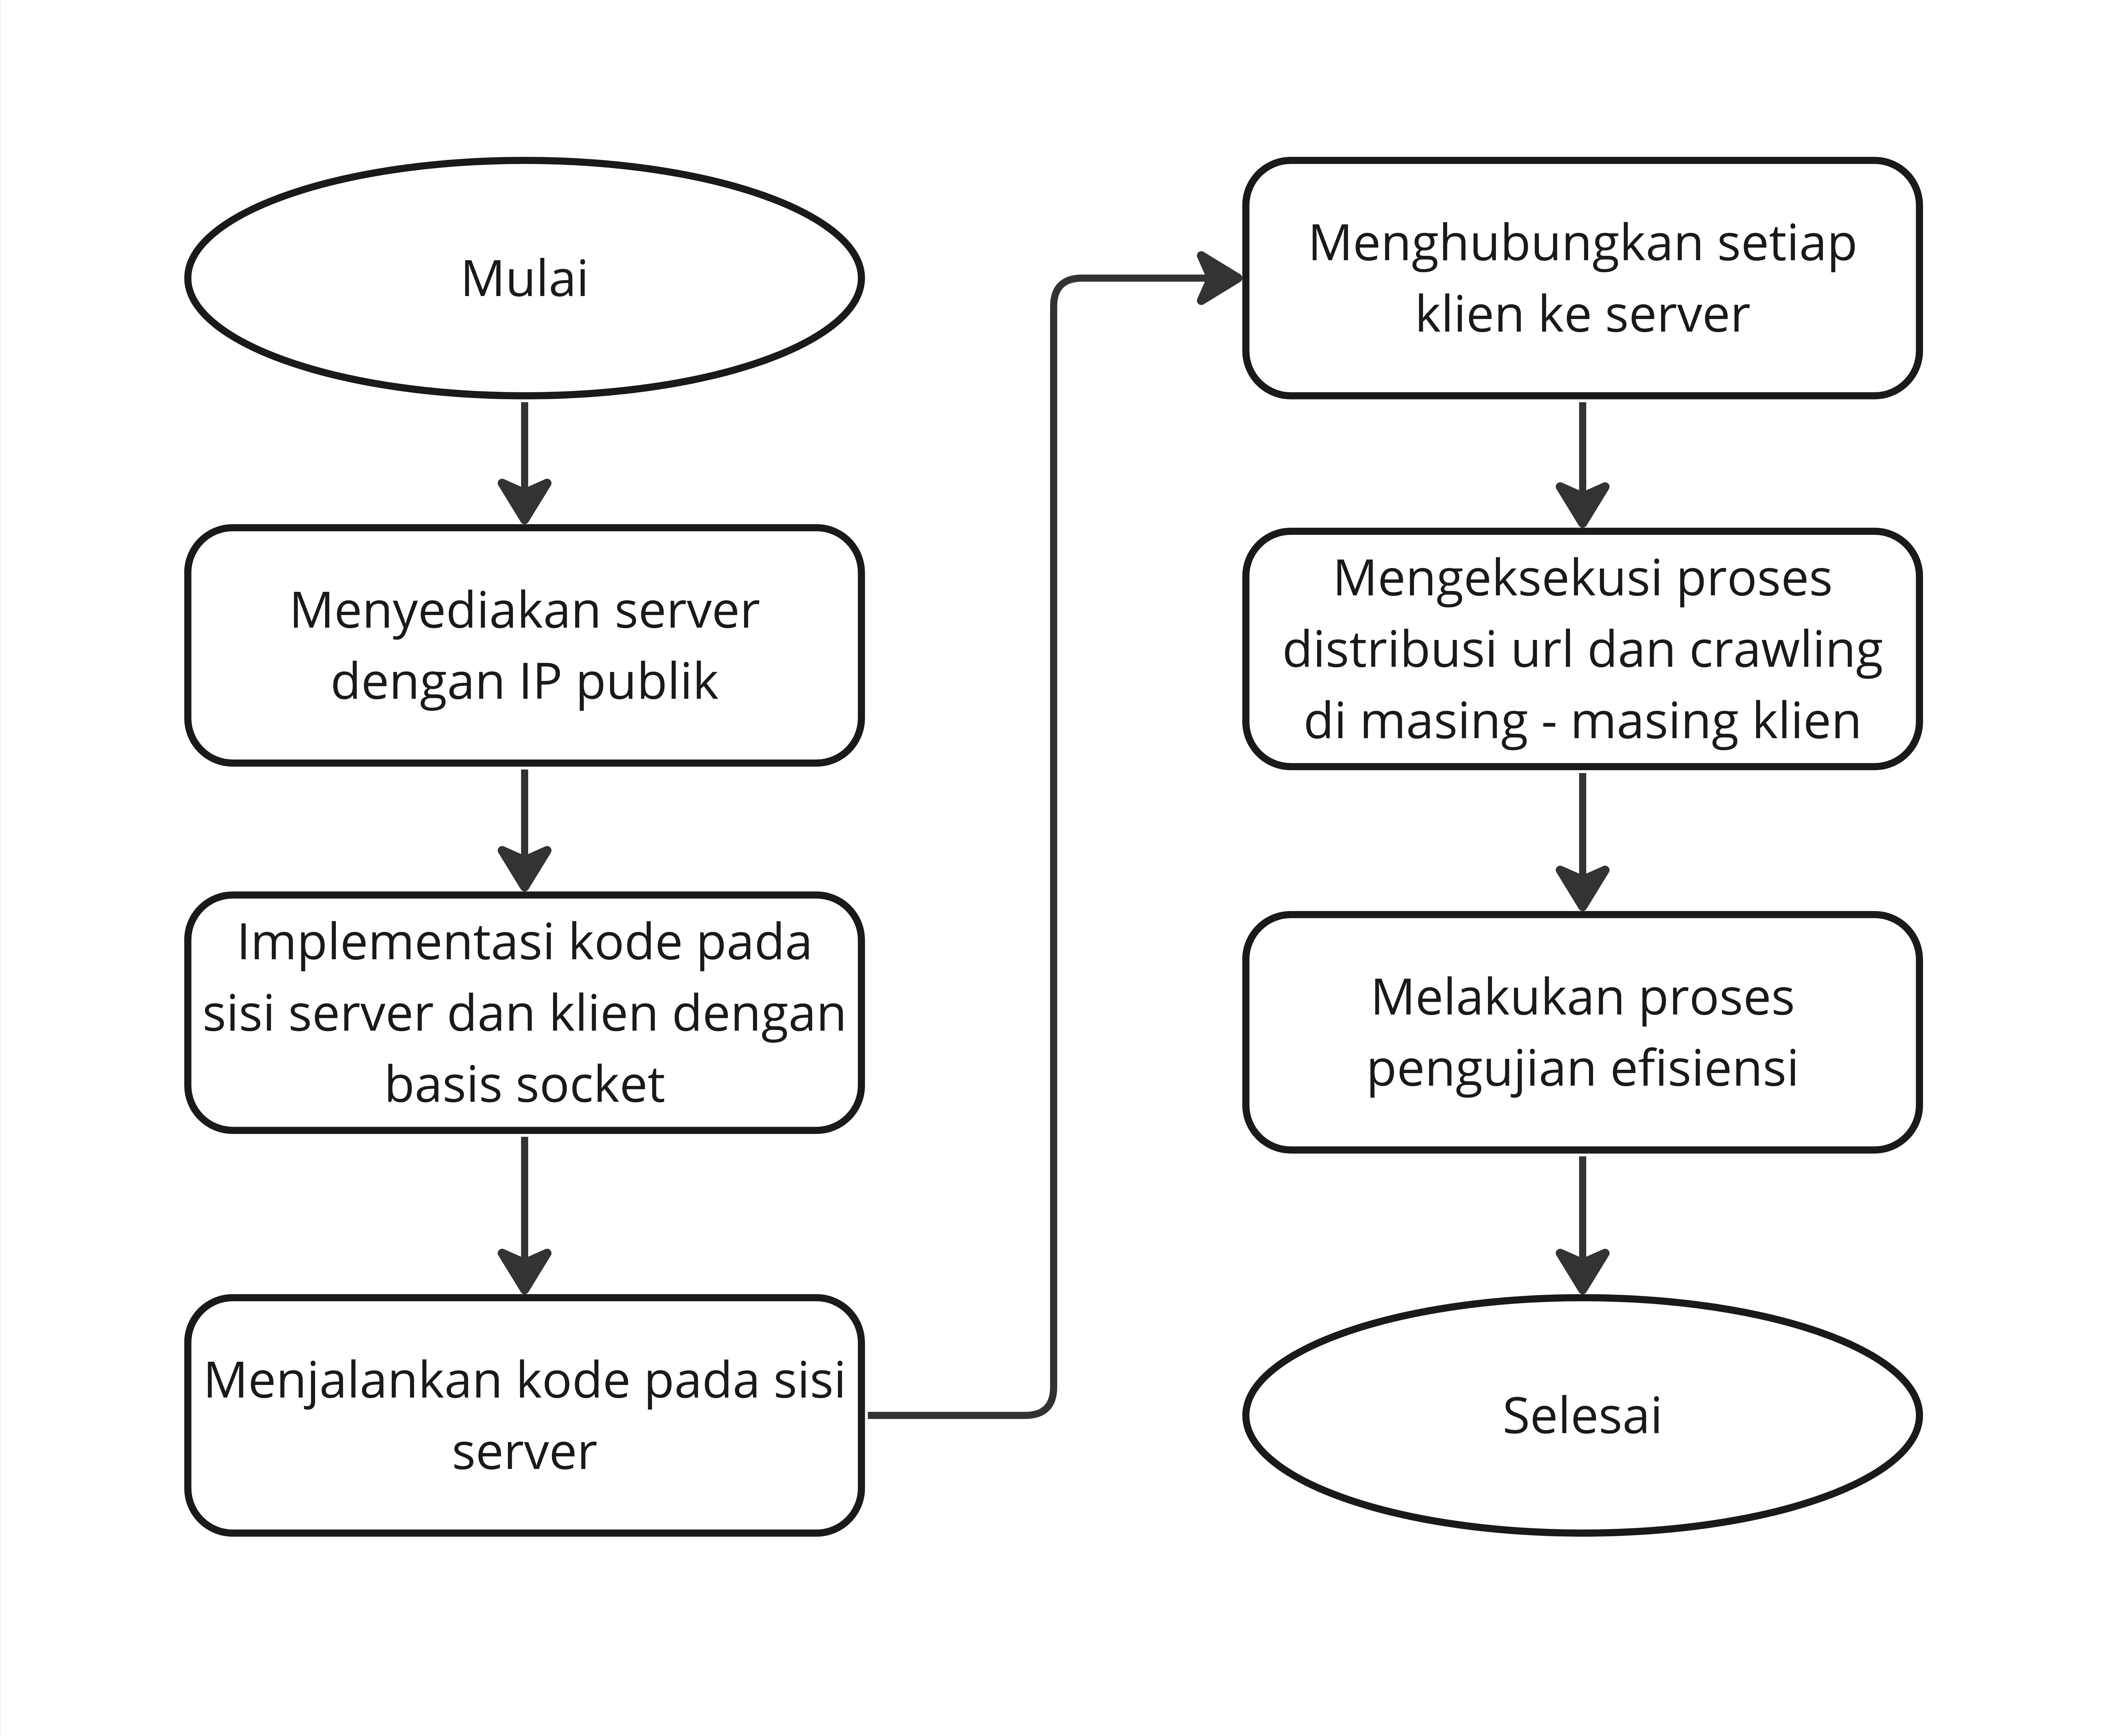
\includegraphics[width=0.6\textwidth]{gambar/flowchart_tahapan_penelitian_crawler_terdistribusi}
  \caption{\emph{Flowchart} Tahapan Penelitian Crawler Terdistribusi}
\end{figure}

Socket berperan penting dalam proses distribusi \emph{url} untuk melakukan crawling pada setiap klien. Karena socket sebagai pokok transportasi url dari satu perangkat ke perangkat yang lain melalui media internet.

Kode program crawler yang ada saat ini hanya menerima masukan url dari perangkat yang menjalankan crawler tersebut. Sedangkan, pada penelitian ini url yang diterima didapatkan dari pembagian dari perangkat lain. Menjadikan klien yang terhubung dapat menjalankan crawling secara bersamaan dan tidak melakukan crawling dengan url yang sama. Jadi tidak ada duplikasi data dari setiap kliennya.

\section{Arsitektur \emph{Crawler} Terdistribusi}

Sistem yang akan dibuat pada penelitian ini adalah pengembangan \emph{crawler} menjadi secara terdistribusi yang dapat berjalan atau melakukan \emph{crawling} pada banyak perangkat sekaligus secara terkontrol. Pengembangan ini menggunakan koneksi socket untuk komunikasi. Gambaran awal arsitektur ini adalah \emph{master-slave}. \emph{Master} bertugas untuk mengelola semua \emph{slave} yang tersedia, melakukan \emph{write operation} ke dalam database, dan membagi serta menyeimbangkan tugas ke masing - masing \emph{slave}. Sedangkan \emph{slave} bertugas untuk melakukan \emph{crawling} dari url yang diberikan oleh \emph{master} dan akan mengembalikan data hasil \emph{crawling} kembali ke \emph{master} untuk dimasukkan ke database, lalu menyeimbangkan kembali url untuk di-\emph{crawling}.

\begin{figure}[H]
  \centering{}
	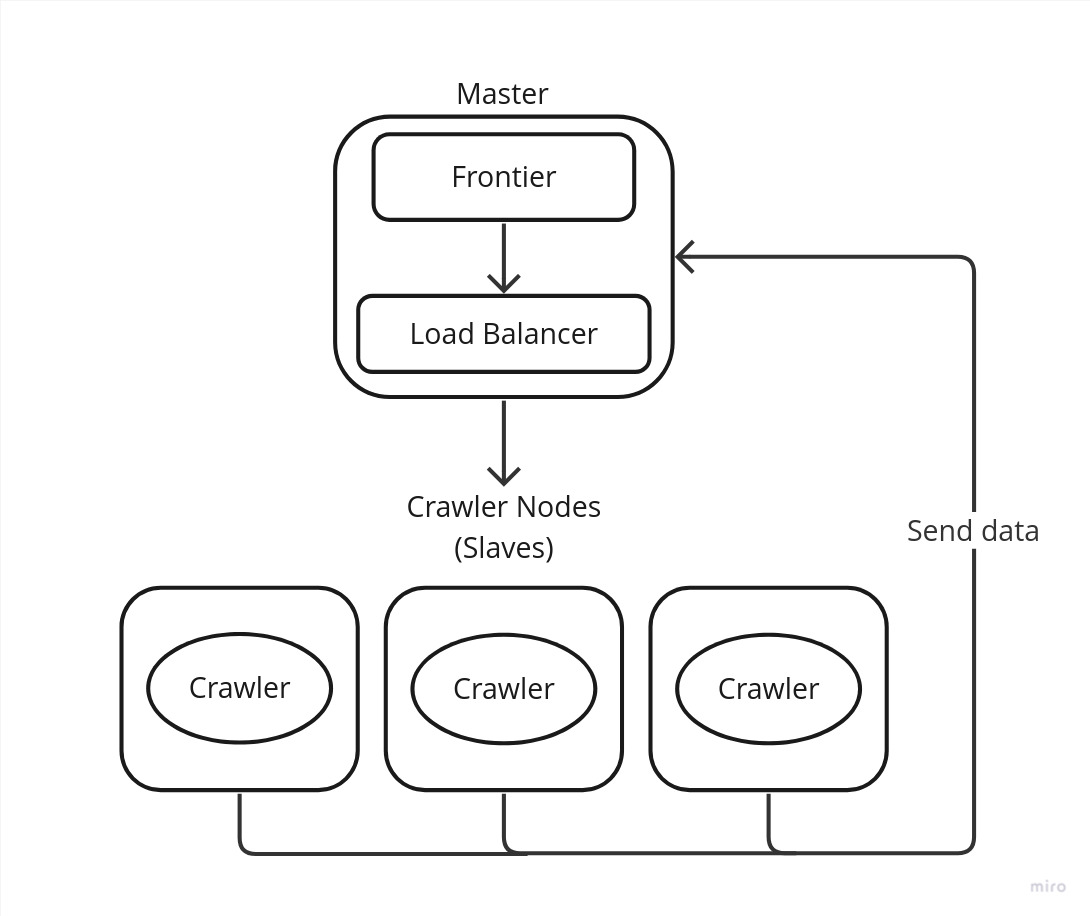
\includegraphics[width=0.6\textwidth]{gambar/crawler_master_slave}
  \caption{Arsitektur \emph{Crawler Master-Slave}}
\end{figure}

\begin{enumerate}
  \item{\emph{Frontier} adalah antrian dari sekumpulan url yang belum dikunjungi dan sudah dikunjungi oleh \emph{crawler}. Url yang terdapat pada \emph{Frontier} sudah terkurasi agar tidak ada url yang terduplikat, guna menghindari melakukan \emph{crawling} pada halaman web yang sama. Kemudian \emph{crawler} akan menerima url dari \emph{frontier} dan melakukan \emph{crawling} pada halaman dari url tersebut.}

  \item{Load balancer bertugas sebagai scheduler untuk mengatur urutan antrian dari url yang akan didistribusikan kepada \emph{crawler}. Mendistribusikan url ke setiap \emph{crawler nodes} agar setiap \emph{crawler} memiliki beban kerja yang seimbang. \emph{Load balancer} memiliki sekumpulan antrian url dari masing - masing \emph{crawler}.}

  \item{\emph{Crawler nodes} adalah perangkat yang akan melakukan \emph{crawler}, url untuk melakukan \emph{crawling} didapatkan dari \emph{frontier} dan hasil dari \emph{crawling} disimpan pada database.}
\end{enumerate}

Berdasarkan arsitektur pada Gambar 3.2, terdapat beberapa pengembangan pada tahapan komunikasi antara \emph{slave} atau klien atau \emph{peer}. Proses komunikasi dilakukan secara langsung antara \emph{peer}, disebut sebagai \emph{peer-to-peer}. Karena komunikasi ini terjadi antara \emph{peer} yang memiliki \emph{private} IP dapat saling berkomunikasi. 

\begin{figure}[H]
  \centering{}
	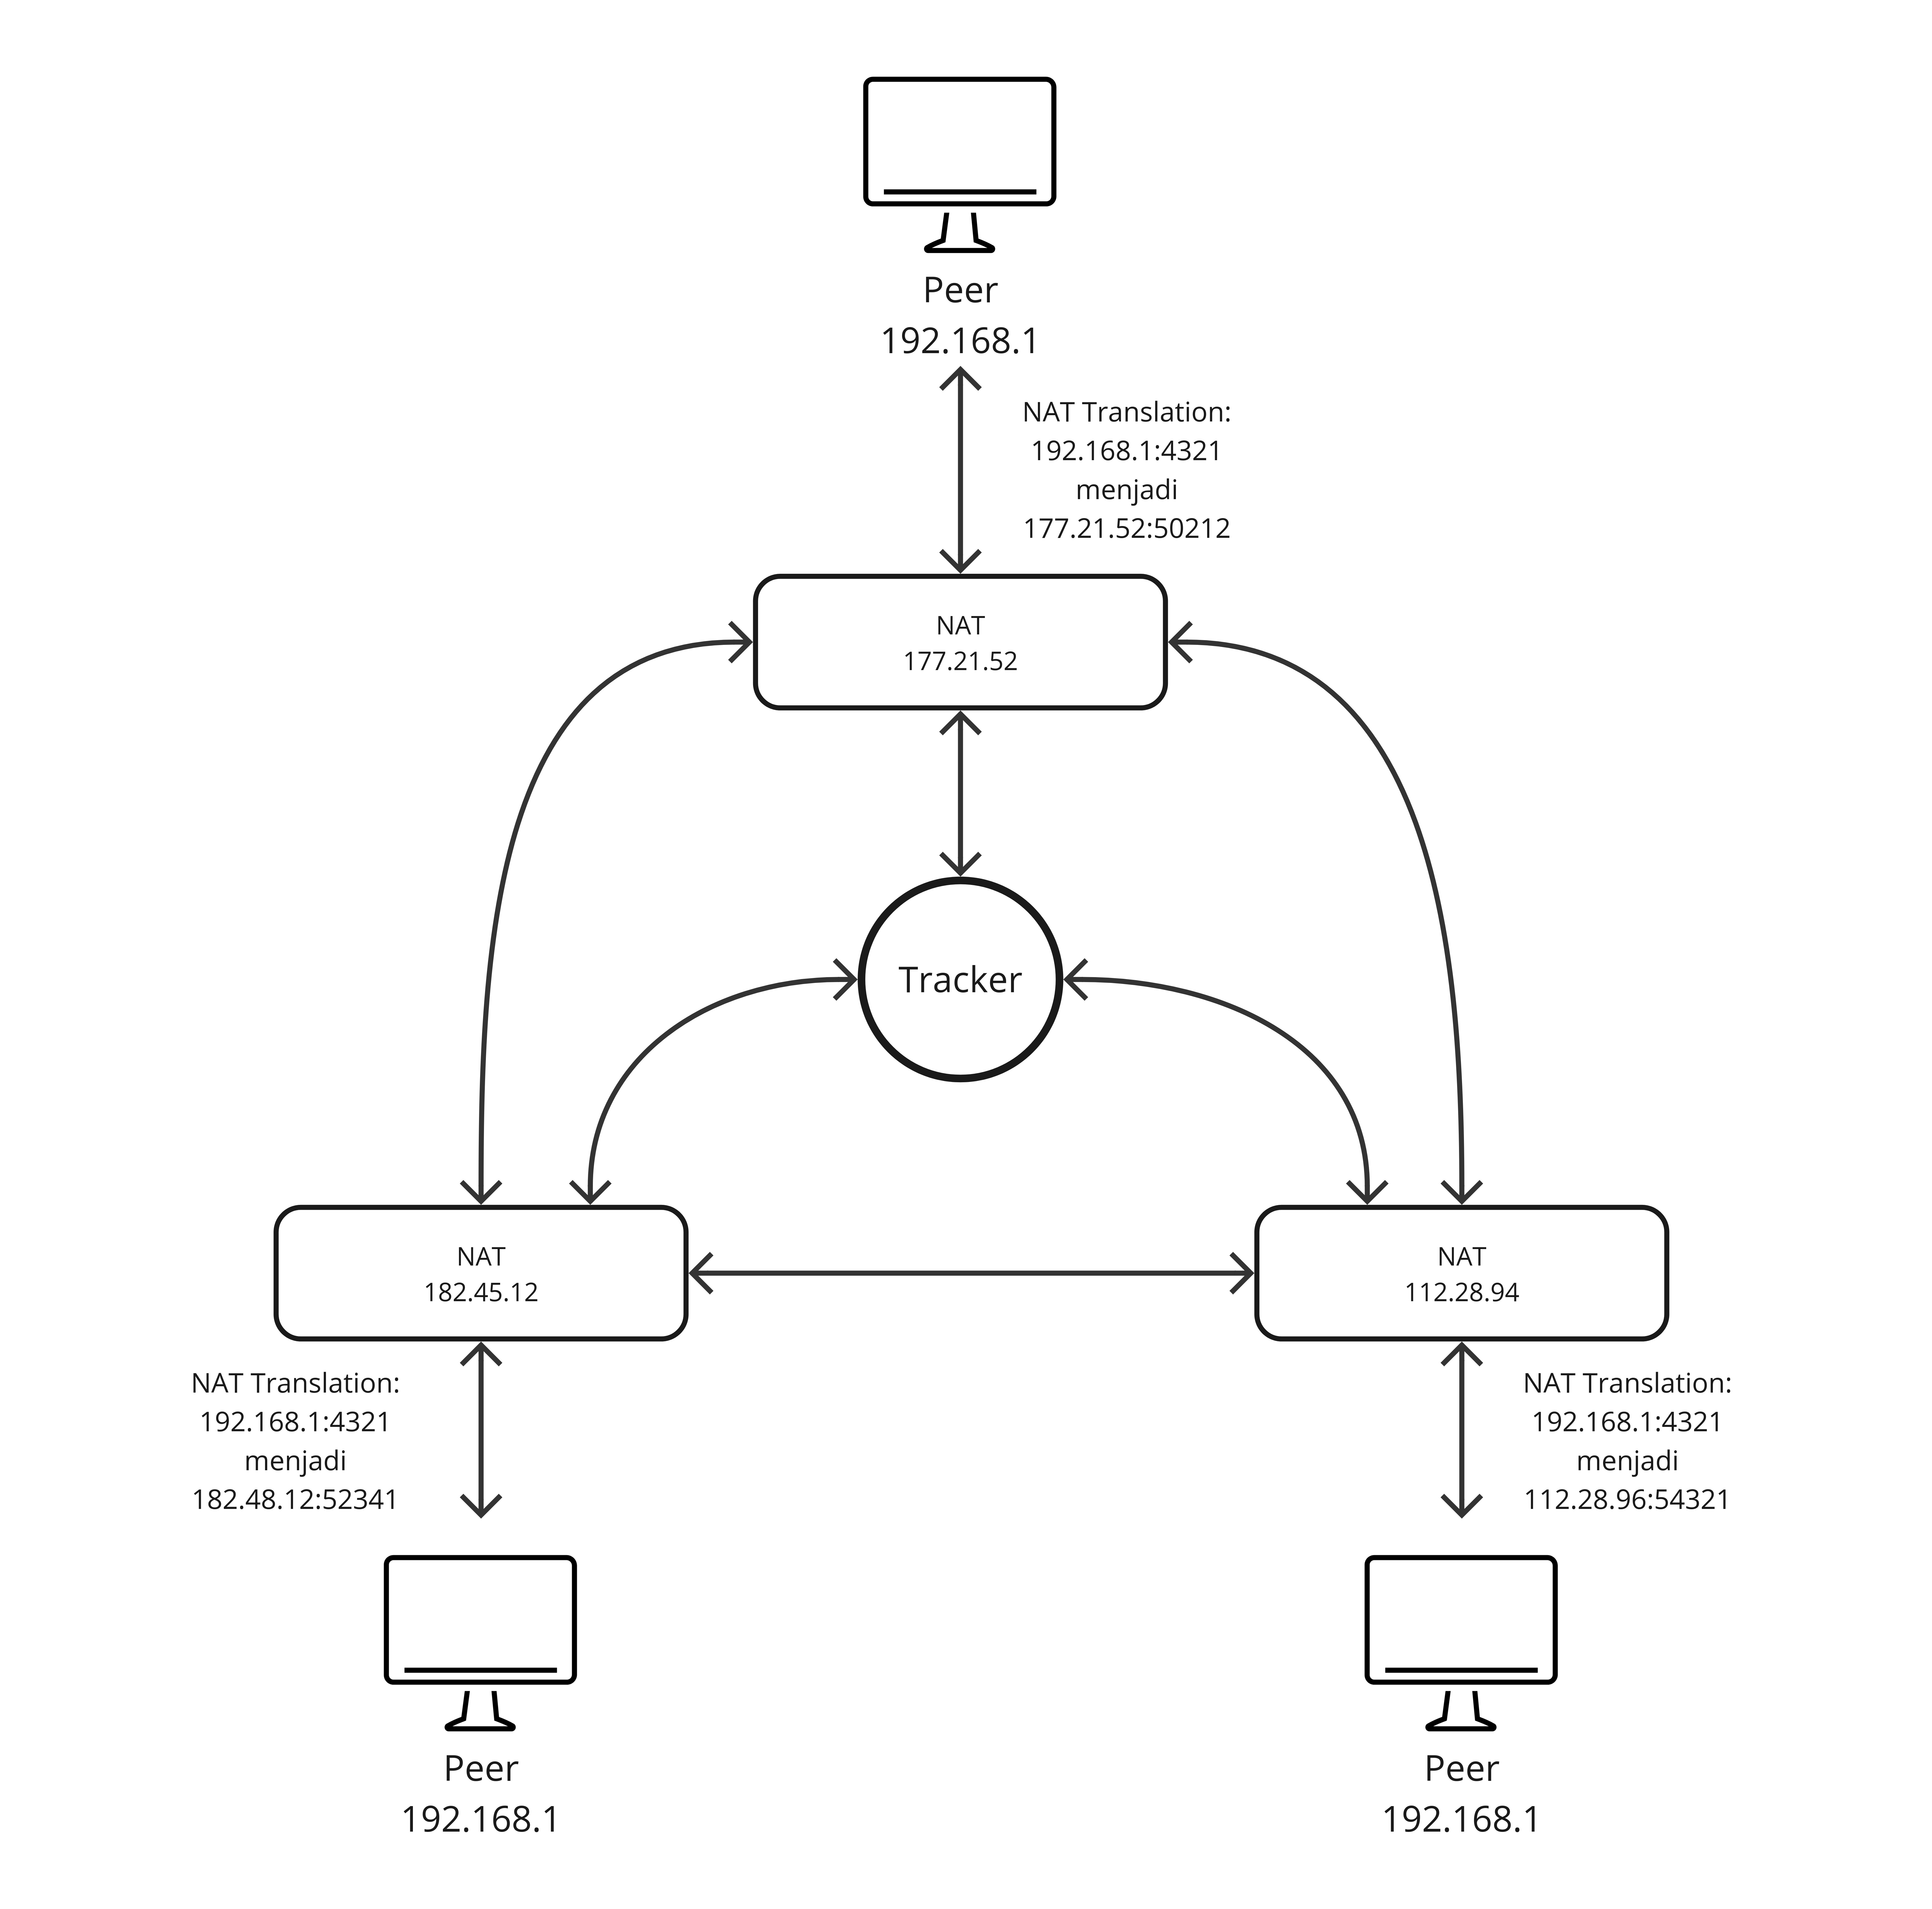
\includegraphics[width=0.6\textwidth]{gambar/peer_to_peer_through_nat}
  \caption{Arsitektur \emph{Crawler Peer to Peer} Melalui NAT}
\end{figure}

\begin{enumerate}
  \item{\emph{Tracker} atau \emph{master} bertugas untuk mengetahui eksternal atau publik IP address dan port dari masing - masing \emph{peer} yang terhubung. \emph{Tracker} adalah sebuah server yang memiliki publik IP. Setelah mengetahui eksternal IP address dan port setiap \emph{peer}, maka \emph{peer} dapat terhubung dengan satu sama lain. Mengoleksi kumpulan \emph{peer} yang terhubung. Setup initial url untuk \emph{crawling}. Melakukan broadcast secara berkala untuk update \emph{peer} yang terhubung dan keluar dari swarm.} 

  \item{\emph{Peer} dapat disebut klien. Setiap \emph{peer} memiliki duplikasi dari kumpulan \emph{peer} yang terhubung dengan \emph{tracker}. Melakukan proses \emph{crawling}. Mengoleksi sekumpulan url untuk di-\emph{crawl}. Mengambil bagian url yang akan di-\emph{crawl} untuk setiap \emph{peer}, saat mengambil url juga mengeluarkannya dari sekumpulan url, sekali mengambil url langsung cukup banyak, bergantung dengan jumlah \emph{peer} yang terhubung, baru di-broadcast kepada semua \emph{peer} yang terhubung atau melalui perantara \emph{tracker} mengenai sekumpulan url yang baru. Minimal menyisakan url lebih banyak dari jumlah \emph{peer} yang terhubung. Agar semua \emph{peer} mendapatkan bagian url yang seimbang. Memasukkan data hasil \emph{crawling} ke database.}
\end{enumerate}

\section{Proses Komunikasi \emph{Peer-to-peer}}

Proses komunikasi menggunakan metode UDP \emph{hole punching}, dengan membuat `lubang' pada NAT, agar antara \emph{peer} dapat saling terhubung antara satu sama lain melalui `lubang' tersebut. Menggunakan socket protokol untuk mengirim packet kepada \emph{tracker} untuk mengetahui publik IP address dari \emph{peer} yang mengirim packet tersebut. Karena \emph{peer} berada di belakang NAT atau router. Jadi IP address dan portnya akan diwakilkan oleh publik IP address dan port dari NAT. Pentingnya untuk mengetahui publik IP address dan portnya, agar \emph{peer} lain dapat terhubung melalui publik IP address dan port dari NAT tersebut. Langkah tersebut dapat dilakukan karena sudah ada “lubang” pada NAT. Ketika \emph{tracker} suatu saat mati dengan sendirinya, proses komunikasi tetap dapat berlanjut, karena transfer data tidak melalui \emph{tracker}. Melainkan menuju langsung ke \emph{peer}.

\begin{algorithm}[H]
  \caption{Algoritma Tracker}\label{alg:peer-to-peer}
  \begin{algorithmic}
    \State $sock.bind('0.0.0.0', port\_number)$ \Comment{Bind socket} 
    \State $clients[]$ \Comment{Inisiasi \textit{clients}}

    \item[] % line skip

    \Function{ListenConnectedPeers}{}
      \While {True}
        \State $data, address \gets sock.recv()$ 
        \State \Call{Append}{$clients[]$, $address$}
      \EndWhile
    \EndFunction

    \item[] % line skip

    \State $listener \gets ListenConnectedPeers()$
    \State $listener.start()$

    \item[] % line skip

    \For{$client \in \mathcal{} clients[..]$}
      \State $address, port \gets \Call{Extract}{$client$} $ 
      \State $sock.sendto(address, port, destination\_address)$
    \EndFor
  \end{algorithmic}
\end{algorithm}

Tracker menjadi sebagai perantara atau \emph{rendezvous} antara klien untuk dapat berkomunikasi di belakang NAT. Tracker akan mengembalikan masing - masing alamat IP dan port dari klien atau \emph{peer} yang terhubung. Dan alamat tersebut bersifat private, karena diwakilkan oleh NAT dari router.

\begin{algorithm}[H]
  \caption{Algoritma Peer}\label{alg:peer-to-peer}
  \begin{algorithmic}
    \State $peers[{address: value, port: value}]$ \Comment{Inisiasi \textit{peers}}
    \State $rendezvous \gets (server_ip, server_port) $
    \State $sock.bind('0.0.0.0', port\_number)$ \Comment{Bind socket} 
    \State $sock.sendto(b'0', rendezvous)$        \Comment{Mengirim pesan kosong ke server} 

    \item[] % line skip

    \Function{ListenPeersFromTracker}{}
      \While {True}
        \State $data \gets sock.recv()$ 
        \State \Call{Append}{$peers[]$, $data$}
      \EndWhile
    \EndFunction

    \State $listenerPeers \gets ListenPeersFromTracker()$
    \State $listenerPeers.start()$

    \item[] % line skip

    \Function{ListenToHolePunch}{}
      \For{$peer \in \mathcal{} peers[..]$}
        \State $address, port \gets \Call{Extract}{$peer$} $ 
        \State $sock.sendto(b'0', port, address)$ \Comment{Proses \emph{hole punch}} 
      \EndFor
    \EndFunction

    \State $listenerHolePunch \gets ListenToHolePunch()$
    \State $listenerHolePunch.start()$

    \item[] % line skip

    \Function{ListenConnectionFromPeers}{}
      \While {True}
        \State $data \gets sock.recv()$  \Comment{Mendapatkan data dari \emph{peer}}
      \EndWhile
    \EndFunction

    \State $listenerConn \gets ListenConnectionFromPeers()$
    \State $listenerConn.start()$

    \item[] % line skip

    \While {True}
      \State $msg \gets input()$ 
      \State $sock.sendto(msg, port, address)$ \Comment{Mengirim data ke \emph{peer} secara spesifik}
    \EndWhile
  \end{algorithmic}
\end{algorithm}

Terdapat proses mengirim pesan kosong ke server, berguna untuk mengetahui alamat IP dan port dari klien yang diwakilkan oleh NAT, karena klien bisa saja memiliki \emph{private} IP dan menyimpannya. Pada fungsi \emph{ListenPeersFromTracker} untuk mendapatkan data alamat dan port dari klien lain, yang nantinya akan digunakan untuk melakukan \emph{hole punching}. Setelah proses itu, kedua atau lebih klien dapat bertukar data secara langsung antara satu sama lain, walaupun klien memiliki \emph{private} IP.

\section{Penyeimbang Antrian \emph{URL}}

Tahapan untuk mengatur urutan antrian url pada \emph{load balancer} terhadap sejumlah \emph{peer} yang tersedia. Setiap \emph{peer} memiliki antriannya sendiri. Gunanya antrian yang berada pada \emph{load balancer} adalah untuk mengatur beban kerja dari \emph{peer}. Agar setiap \emph{peer} mendapatkan tugas yang seimbang untuk melakukan crawling. Ketika salah satu \emph{peer} memiliki antrian url yang banyak dan tidak seimbang dengan \emph{peer} yang lain. Maka url yang berasal dari frontier akan diantrikan ke \emph{peer} yang lain dengan jumlah antrian yang lebih sedikit.

% \begin{figure}[H]
%   \centering{}
% 	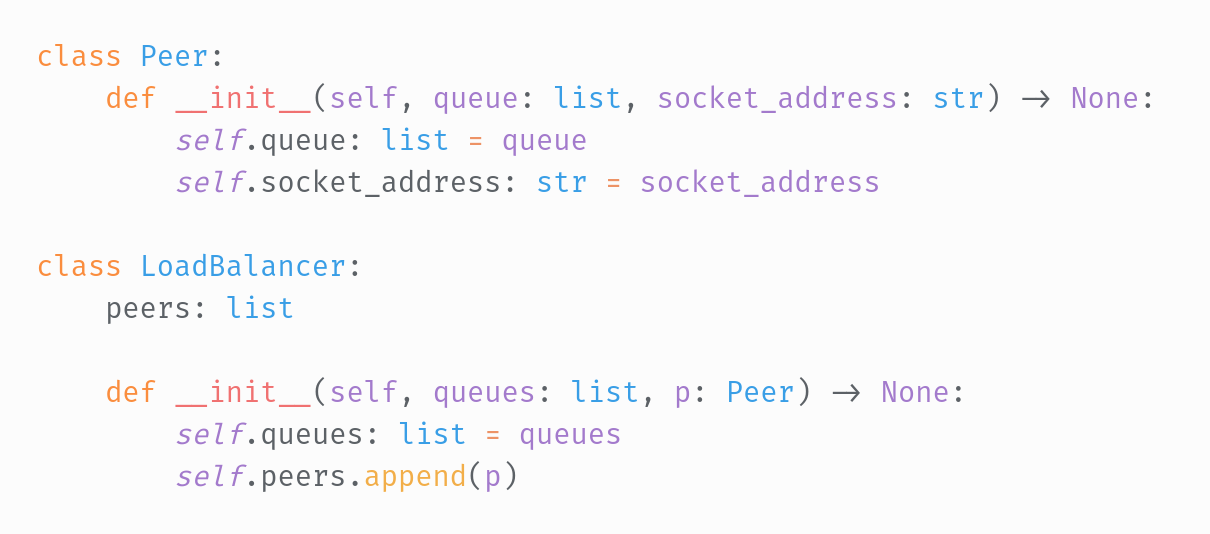
\includegraphics[width=1\textwidth]{gambar/struktur_data}
%   \caption{Penulisan struktur data pada \emph{Python}}
% \end{figure}

\begin{algorithm}[H]
  \caption{Struktur Data}\label{alg:peer-to-peer}
  \begin{algorithmic}
    \Struct{Peer} {queue: list, socket\_address: str}
      \State $self.queue \gets queue$
      \State $self.socket\_address \gets socket\_address$
    \EndStruct

    \item[] % line skip

    \Struct{LoadBalancer} {queues: list, p: Peer}
      \State $self.queues \gets queues$
      \State $self.peers.\textbf{append}(p)$
    \EndStruct
  \end{algorithmic}
\end{algorithm}



\begin{algorithm}[H]
  \caption{Algoritma Penyeimbang Antrian}\label{alg:peer-to-peer}
  \begin{algorithmic}
    \State $balancer = LoadBalancer$
    \State $queues = balancer.queues$

    \item[] % line skip

    \Function{BalancingQueue}{$list\_of\_url$}
      \For{$url \in \mathcal{} list\_of\_url[..]$}
        \State $min\_length = INFINITY$
        \State $min\_queue\_index = None$
        
        \item[] % line skip

          \For{$i, current\_queue \in enumerate(queues[..])$}
            \State $current\_length = current\_queue.length()$
              \If{$current\_length == 0$}
                \State $min\_queue\_index = i$
                \State $break$
              \ElsIf{$current\_length < min\_length$}
                \State $min\_length = current\_length$
                \State $min\_queue\_index = i$
              \EndIf
          \EndFor
      \EndFor

      \State $queues[min\_queue\_index].enqueue(url)$
    \EndFunction
  \end{algorithmic}
\end{algorithm}

\section{Skema Pendistribusian}

\begin{figure}[H]
  \centering{}
	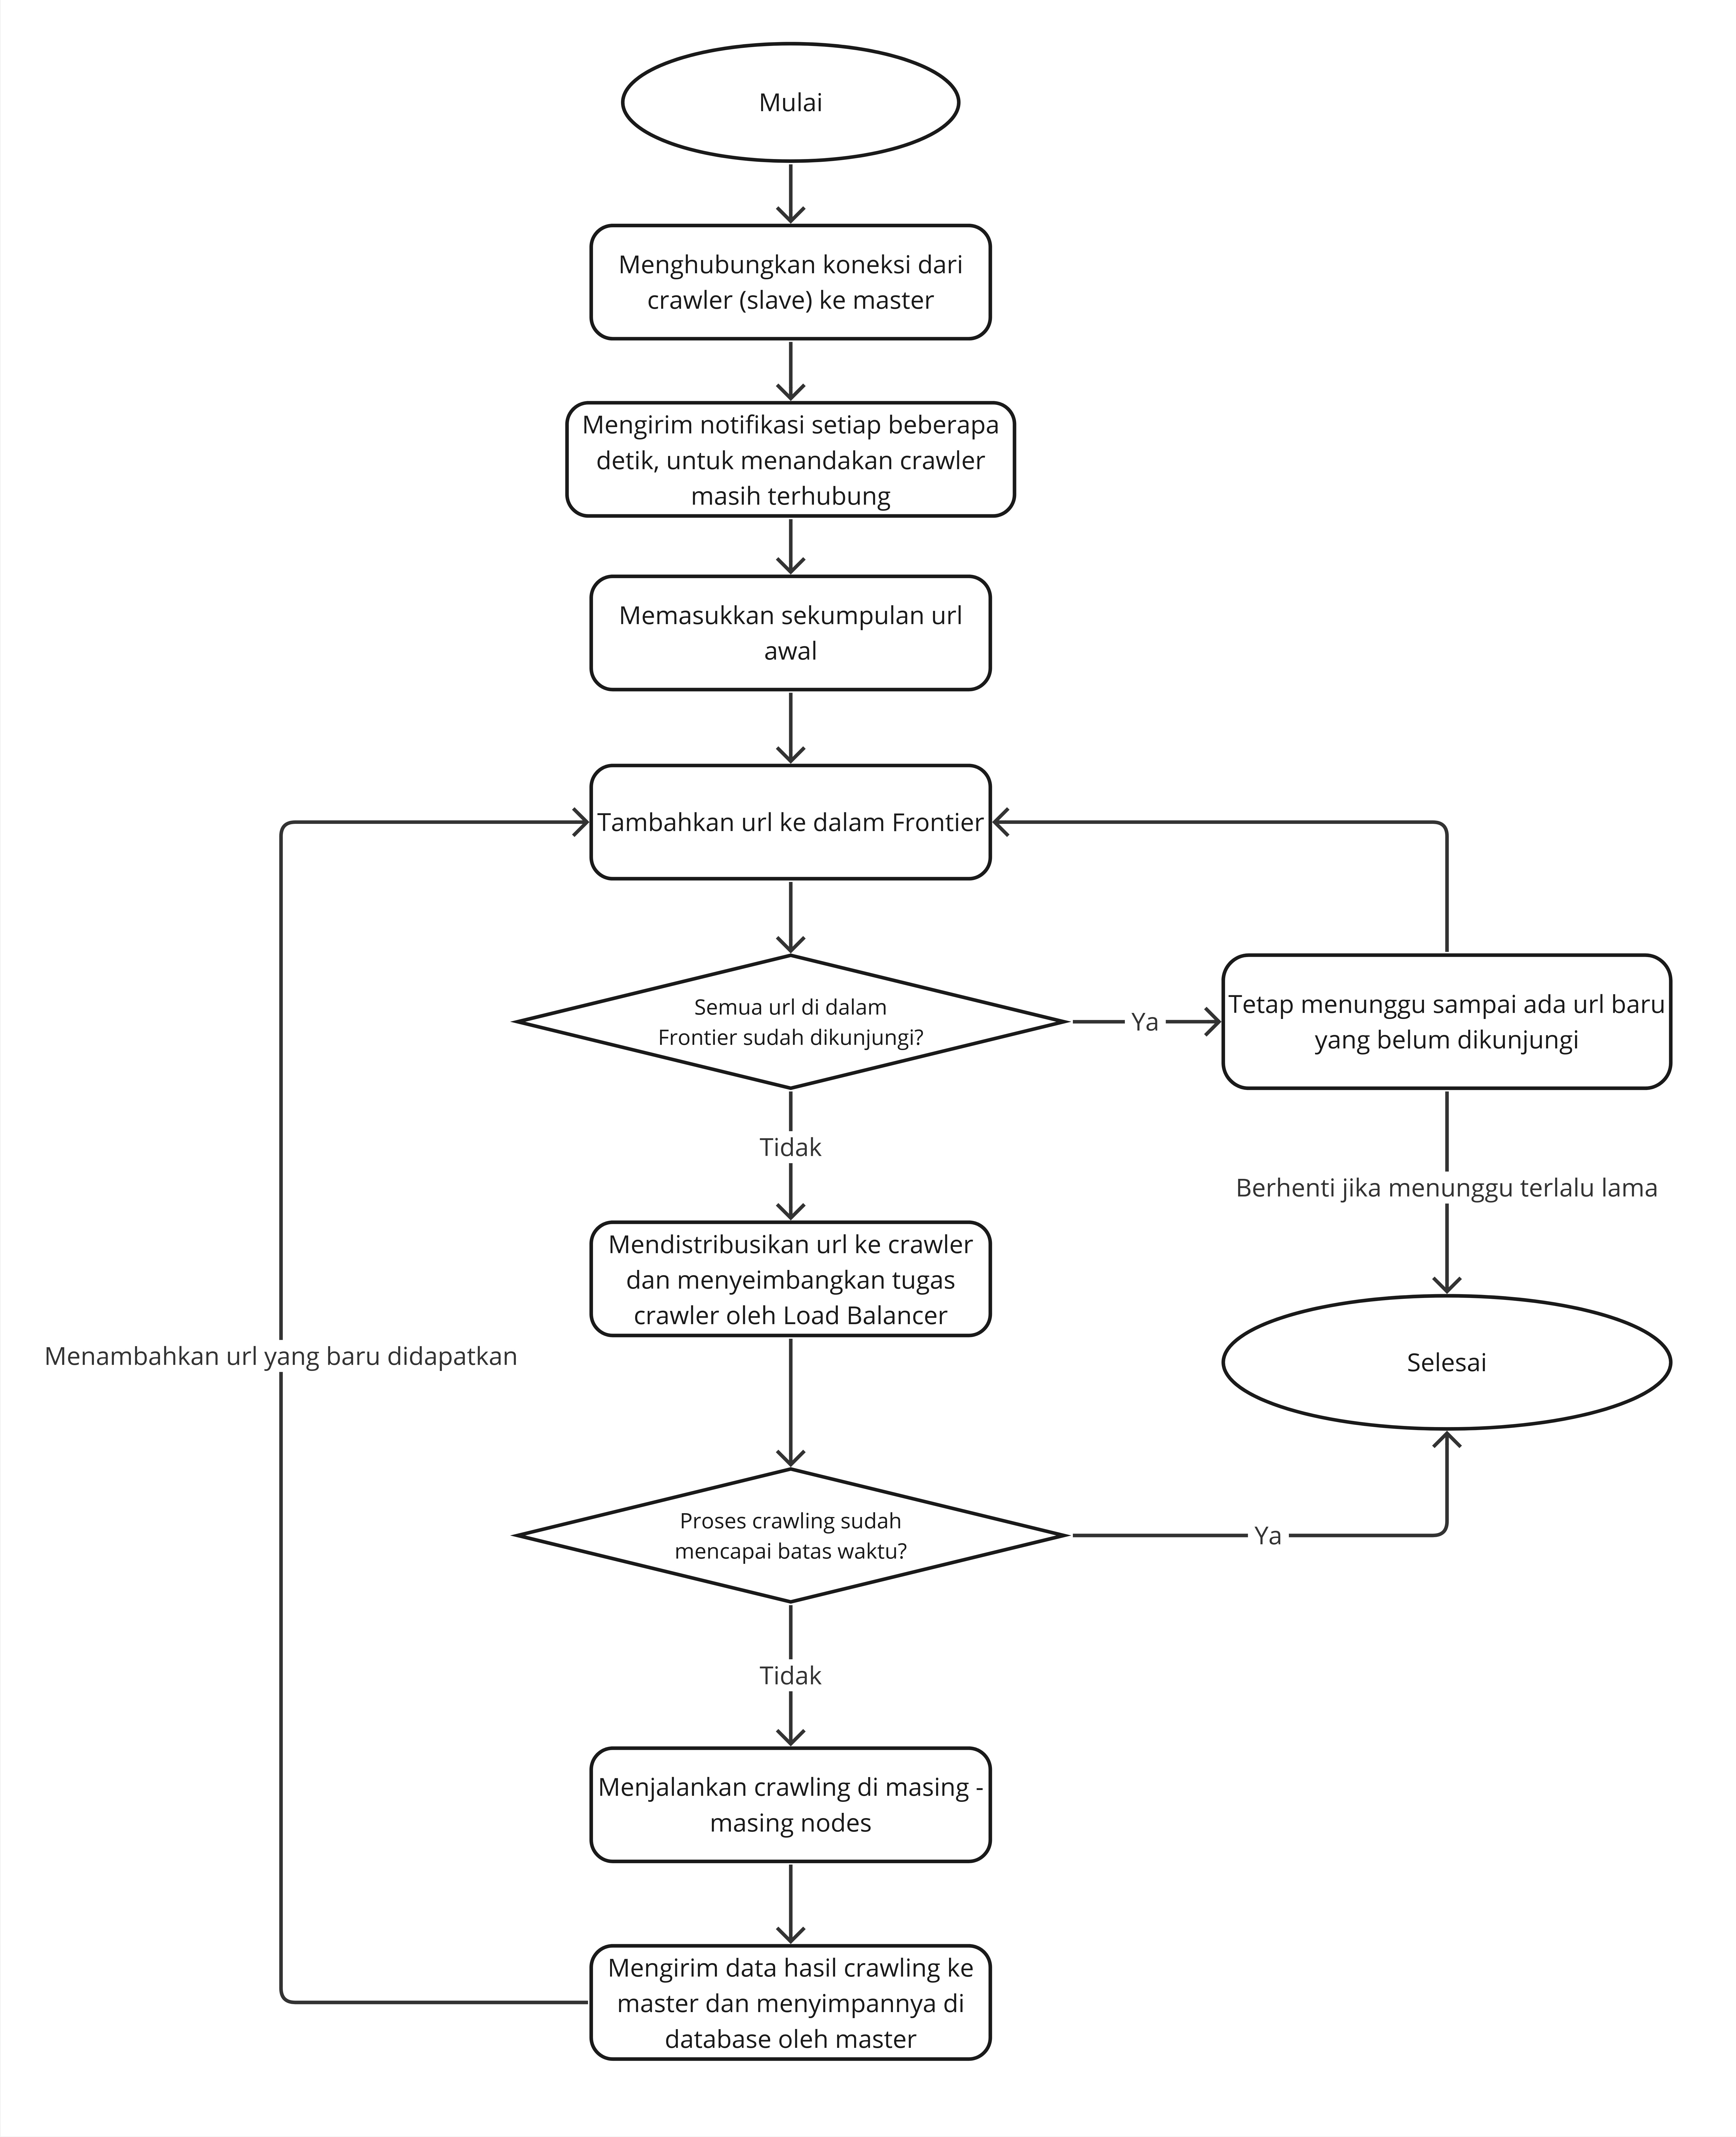
\includegraphics[width=1\textwidth]{gambar/flowchart_distributed_crawler}
  \caption{\emph{Flowchart} Skema Pendistribusian}
\end{figure}

Proses dari sistem \emph{crawler} terdistribusi dimulai dengan memasukkan sekumpulan url awal yang ingin di-\emph{crawling} ke dalam \emph{frontier}. Lalu, melakukan pengecekan terhadap url yang sudah dikunjungi di \emph{frontier}. Jika kondisinya tidak, maka akan melanjutkan untuk mendistribusikan url ke masing - masing \emph{crawler} dan menyeimbangkan beban kerjanya. Setelah itu melakukan \emph{crawling} oleh \emph{crawler} dan data disimpan di database. Data yang didapatkan dari \emph{crawling} akan dikembalikan ke \emph{frontier} yang berbentuk outgoing url dan akan dilakukan penyaringan url yang belum dikunjungi. Ketika kondisi semua url pada \emph{frontier} sudah dikunjungi maka akan menunggu sampai ada url baru yang belum dikunjungi. Akan \emph{suspend} ketika terlalu lama menunggu.

\section{Alat dan Bahan Penelitian}

Pada penelitian ini, terdapat beberapa alat yang digunakan sebagai penunjang
dalam pembuatan sistem terdistribusi dengan rincian sebagai berikut:

\begin{itemize}
  \item{Dua laptop dengan konfigurasi Intel Core i7-8650U, 16GB RAM dan Intel Core i5-8265U, 20GB RAM}
  \item{Sistem operasi \textit{Linux}}
  \item{\textit{VSCode} sebagai \textit{code editor}}
  \item{Database \textit{SQLite3} untuk menyimpan data}
  \item{\textit{Python 3}}
  \item{\textit{Virtual private server} untuk menjalankan program yang memerlukan public IP address}
\end{itemize}

\section{Tahapan Pengembangan}

\subsection{Improvisasi \emph{crawling} secara terdistribusi}

Proses improvisasi akan dilakukan dengan memodifikasi \emph{crawler} agar dapat berjalan secara terdistribusi, serta meningkatkan konsistensi data dan efisiensi sumber daya. Penelitian ini akan mengembangkan versi \emph{crawler} terdahulu (\cite{lazuardy2023search}). 

Hasil penelitian tersebut menghasilkan \emph{crawler} yang dapat menghimpun data dari bebagai halaman \emph{web} dengan tambahan \emph{multi-threading} yang dapat memaksimalkan proses kerja dengan membagi pekerjaan ke \emph{thread} yang lain. Karena hasil penelitian sebelumnya masih berjalan dalam satu perangkat saja. Dan tidak dapat berkoordinasi dengan perangkat lain. Maka, penelitian ini akan mengembangkan menjadi terdistribusi dengan mekanisme \emph{socket programming}.

\subsection{Skenario Eksperimen}

Berikut adalah skenario eksperimen agar perangkat dapat berkomunikasi satu sama lain dengan \emph{socket} dan melakukan \emph{crawling}.

\begin{enumerate}
  \item{Menjalankan program tracker pada server dengan public IP}
  \item{Menjalankan program manager pada server dengan public IP. Dan terhubung ke tracker}
  \item{Menjalankan program klien, pada server dengan public IP dan ada juga yang berjalan di private IP nantinya klien akan terkurasi yang memiliki IP public dan private. Dan terhubung ke tracker}
  \item{Manager melakukan binding koneksi, agar klien public dapat terhubung kepadanya dengan mengirim info ke tracker}
  \item{Tracker menginformasi klien public untuk mencoba terhubung ke manager dengan memberikan IP address dan portnya}
  \item{Klien public menerima informasi tersebut dan menghubungkan koneksi ke manager}
  \item{Setelah berhasil, klien public akan melakukan binding koneksi agar semua klien private dapat terhubung dengannya. Lalu memberikan informasi kepada tracker terkait hal itu}
  \item{Tracker menginformasi semua klien private untuk mencoba terhubung ke klien public dengan memberikan IP address dan portnya}
  \item{Klien private menerima informasi tersebut dan menghubungkan koneksi ke klien public}
  \item{Manager mengirim starting url yang diperlukan kepada klien public yang terhubung}
  \item{Klien public menerima starting url dan mengirimkan kepada klien private (yang aka melakukan \emph{crawling})}
  \item{Klien private melakukan \emph{crawling} dan setiap selesai satu url. Data hasilnya (konten dari web yang di-\emph{crawl} dan sekumpulan url baru yang ditemukan) akan dikirimkan ke klien public}
  \item{Klien public akan menyimpan data konten hasil \emph{crawling} di database. Dan sekumpulan url yang didapat akan dicek apakah ada duplikasi atau tidak}
  \item{Klien public kembali mengirim url yang akan di-\emph{crawling} kepada semua klien private dengan mempertimbankan "kesehatan" dari klien tersebut dan jumlah url yang berada di klien itu. Agar pembagian menjadi seimbang}
\end{enumerate}

\section{Skema Uji}

Pengujian yang akan dilakukan pada penelitian ini adalah untuk menguji konsistensi data dan efisiensi dengan crawler terdahulu.

\subsection{Sumber Data}

Sumber data yang akan digunakan dalam penelitian ini adalah situs web berita dan data yang diambil itu mencakup konten teks dari halaman web serta tautan yang berada di web tersebut.

\subsection{Metrik Pengujian}

Performa crawler terdistribusi akan dinilai menggunakan metrik berikut:
\begin{enumerate}
  \item{\textbf{Proses Komunikasi}: Proses komunikasi antara masing - masing perangkat dapat berjalan dengan sistematis.}

  \item{\textbf{Konsistensi Data}: Konsistensi data mengacu pada kemampuan mengirimkan data lengkap tanpa kehilangan atau duplikasi informasi  selama proses \emph{crawling}. Konsistensi data penting untuk memastikan keakuratan dan kelengkapan informasi yang dikumpulkan di Internet. Duplikasi atau hilangnya data dapat menyebabkan analisis yang tidak akurat dan berdampak pada keputusan berdasarkan data tersebut. Dengan pengujian analisis data tersimpan dengan membandingkan data yang dikumpulkan dengan sumber atau data yang diharapkan untuk memastikan tidak ada duplikasi.}
    
  \item{\textbf{Efisiensi dan Optimalisasi}: Efisien sumber daya dan optimalisasi jumlah data yang terkumpul dari proses \emph{crawling} terdistribusi dengan \emph{crawling} tidak terdistribusi. Ini mencakup seberapa cepat sistem dapat mengumpulkan data. Karena proses crawling yang lambat atau penggunaan sumber daya yang tidak efisien dapat menghambat kinerja \emph{crawler}. Dengan pengujian penyimpanan data, data yang dihasilkan oleh \emph{crawler} terdistribusi dapat memiliki jumlah data yang lebih banyak dalam kurun waktu yang sama, yaitu satu jam.}
\end{enumerate}

\subsection{Rancangan Eksperimen}

\begin{enumerate}
  \item{Menjalankan kedua versi crawler secara bersamaan dengan \emph{initial url web} yang sama.}
  \item{Catat jumlah data yang terkumpul dalam jangka waktu tertentu}
\end{enumerate}

% \subsection{Batasan Pengujian}

% Pengujian ini memiliki batasan pada durasi \emph{crawling} dan tidak mempertimbangkan faktor-faktor seperti kondisi jaringan yang bervariasi.

% \subsection{Implikasi Hasil}

Skema uji ini akan membantu dalam membandingkan kinerja antara crawler terdistribusi dan terdahulu (tanpa terdistribusi).
% Frontier dan \emph{load balancer} terletak pada suatu mesin yang disebut master machine. Dan untuk setiap \emph{crawler} berada pada mesin yang disebut sebagai slaves machine. Slaves machine dapat terdiri lebih dari satu. Setiap slave machine terhubung dengan master machine melalui koneksi socket.
